%!TEX root = ../template.tex
%%%%%%%%%%%%%%%%%%%%%%%%%%%%%%%%%%%%%%%%%%%%%%%%%%%%%%%%%%%%%%%%%%%%
%% chapter5.tex
%% NOVA thesis document file
%%
%% Chapter with lots of dummy text
%%%%%%%%%%%%%%%%%%%%%%%%%%%%%%%%%%%%%%%%%%%%%%%%%%%%%%%%%%%%%%%%%%%%

\typeout{NT FILE chapter5.tex}%

\chapter{Metodologia Proposta}
\label{cha:metodologia_proposta}

Neste tópico é abordado a metodologia proposta para o projeto, de forma a projetar um plano de trabalho para o trabalho que se segue na implementação do \textit{Dittor}, mencionando possíveis ajudas, testes de implementação e discussão de resultados.

\section{Contacto frequente com Tor's Network Health Team}
\label{sec:contacto_team}

Visto existir um contacto constante com a \textit{Network Health Team} do Tor desde o início deste projeto, que ajudou a direcionar e a suportar com explicação de uma linha de trabalho passada por onde havia caminho por explorar, o objetivo é manter esta ligação de modo a que este projeto vá de encontro às necessidades do Tor, para que mais tarde possa ser implementado ou até usado para futuras implementações.

A equipa de \textit{Network Health} não só disponibilizou-se para futuras reuniões e contactos diretos como mostrou-se interessada nos resultados do projeto, o que facilita na organização de prioridades e objetivos com o mesmo.

\section{Test Case na FCT}
\label{sec:testcase_fct}

Um dos objetivos delineados explora a implementação do \textit{Dittor} num ambiente controlado, de forma a averiguar resultados do sistema numa rede que simula o Tor. Para tal, seria possível, com autorização do Departamento de Informática da NOVA FCT, o uso de tecnologias de \textit{shadow software} no \textit{cluster} da universidade, de forma a não consumir muitos recursos do mesmo mas simulando uma pequena rede Tor, com \textit{Directory Authorities} e circuitos integrados, que usasse o projeto de forma a construir um ambiente que seja razoavelmente parecido e que produzisse resultados semelhantes, mas a escala pequena.

Para testar a mitigação de \textit{Sybil attacks}, ferramentas para teste de sistemas e injeção de \textit{sybils} \cite{sendner2025impact} seria o ideal, de forma a simular de forma mais realista os resultados provenientes de defesa contra este tipo de ataques.

\section{Discussão de Resultados e Demonstração no Tor}
\label{sec:discussao}

Para avaliar a solução implementada, serão utilizados os requisitos enunciados no início do projeto. A partir dos mesmos, é possível implementar requisitos que promovem a discussão científica dos resultados obtidos, avaliando a solução tanto ao nível de \textit{performance} como na segurança, mais concretamente na mitigação de \textit{Sybil attacks}.

A partir dos resultados e conclusões retiradas futuramente, está como objetivo adicional do projeto, mediante resultados positivos e aprovação superior do \textit{The Tor Project}, a implementação momentânea do \textit{Dittor} na rede Tor, de forma a testar o seu funcionamento num cenário real. Isto não passa de objetivo para já, visto que para obter aprovação do \textit{The Tor Project} para implementação é necessário obter primeiro os resultados, que advêm da implementação do \textit{Dittor}, embora tenha sido um assunto discutido em reuniões com a equipa de \textit{Network Health}.

\section{Gantt Chart}
\label{sec:gantt}

Para projeção do cronograma de fases de implementação ao longo do projeto, cria-se um \textit{Gantt Chart} para visualização intuitiva:

\begin{figure}[H]
    \centering
    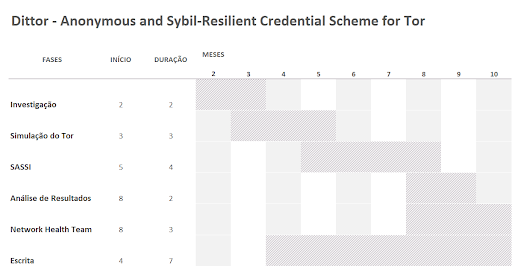
\includegraphics[width=0.7\linewidth]{5-Figures/GanttChart.png}
    \caption{Cronograma das fases de implementação do projeto.}
    \label{fig:ganttchart}
\end{figure}

Este projeto começa pela fase da \textbf{Investigação}, que engloba toda a procura de artigos e conhecimento relativo ao início da implementação de um ambiente informático simulador da rede Tor e do sistema de credenciais do \textit{SASSI}, desde implementações passadas de ambos a artigos científicos que auxiliem o processo. Esta fase tem uma duração de dois meses, de forma a delinear um plano de implementação e passos para auxílio do processo. De seguida, a \textbf{Simulação do Tor} e o \textbf{SASSI} contemplam a implementação do ambiente de testes a partir do conhecimento obtido na \textbf{Investigação}, de forma a simular uma rede de utilizadores para obtenção de resultados fidedignos, que tem uma duração expectada de sete meses, sendo o obstáculo principal do projeto e as fases mais demoradas, englobando os pedidos de permissões de uso do \textit{cluster} da NOVA FCT e potenciais passos burocráticos. 

A fase da \textbf{Análise de Resultados} constitui dois meses de procura de requisitos e formulação de gráficos para visualização simplificada dos resultados obtidos, que decorre simultaneamente com apoio da \textbf{Network Health Team} do Tor para entender os mecanismos adequados para medição do nível de sucesso do projeto, de forma a desenvolver uma implementação útil para o futuro do Tor. Esta última fase tem uma duração estimada de três meses, para perguntas e respostas com auxílio da equipa do Tor.

Por último, a fase da \textbf{Escrita} contempla a escrita da tese e projeto final, que deverá ter início em abril, para começar a delinear a estrutura do projeto com antecedência e completando à medida que as fases vão avançando.